\documentclass[11pt]{article}
\usepackage[utf8]{inputenc}
\usepackage[T1]{fontenc}     % Fix weird character
\usepackage{geometry}
\usepackage{amsmath}
\usepackage{amssymb}
\usepackage{gensymb}
\usepackage{spalign}
\usepackage{xfrac}
\usepackage{parskip}
\usepackage{float}  % figure[H]
\usepackage[english]{babel}
\usepackage[style=ieee,backend=biber,urldate=iso,date=iso]{biblatex}
\usepackage[breaklinks=true,bookmarks=true,hidelinks]{hyperref}
\usepackage{tikz}
\usepackage{pgfplots}
\usepackage[yyyymmdd]{datetime}
\usepackage{booktabs}
\usepackage{graphicx}
\usepackage[skip=0.5\baselineskip]{caption}
\usepackage{varwidth}
\pgfplotsset{compat=newest,compat/show suggested version=false}

\geometry{
    a4paper,
    hmargin=2.54cm,
    tmargin=1.27cm,
    bmargin=1.27cm,
    includeheadfoot
}
\setcounter{secnumdepth}{0}  % Disable section numbering

\begin{filecontents}{doit.bib}
@misc{wiki:osi,
    author = "{Wikipedia contributors}",
    title = "OSI model --- {Wikipedia}{,} The Free Encyclopedia",
    year = "2024",
    url = "https://en.wikipedia.org/w/index.php?title=OSI_model&oldid=1219778555",
    note = "[Online; accessed 24-April-2024]"
}
@misc{wiki:vas,
    author = "{Wikipedia contributors}",
    title = "Virtual address space --- {Wikipedia}{,} The Free Encyclopedia",
    year = "2024",
    url = "https://en.wikipedia.org/w/index.php?title=Virtual_address_space&oldid=1218215420",
    note = "[Online; accessed 28-April-2024]"
}
@misc{wiki:havard,
    author = "{Wikipedia contributors}",
    title = "Harvard architecture --- {Wikipedia}{,} The Free Encyclopedia",
    year = "2024",
    url = "https://en.wikipedia.org/w/index.php?title=Harvard_architecture&oldid=1197202451",
    note = "[Online; accessed 28-April-2024]"
}
@misc{wiki:von,
    author = "{Wikipedia contributors}",
    title = "Von Neumann architecture --- {Wikipedia}{,} The Free Encyclopedia",
    year = "2024",
    url = "https://en.wikipedia.org/w/index.php?title=Von_Neumann_architecture&oldid=1218402813",
    note = "[Online; accessed 28-April-2024]"
}
@misc{wiki:forwardingtable,
    author = "{Wikipedia contributors}",
    title = "Forwarding information base --- {Wikipedia}{,} The Free Encyclopedia",
    year = "2023",
    url = "https://en.wikipedia.org/w/index.php?title=Forwarding_information_base&oldid=1159651747",
    note = "[Online; accessed 28-April-2024]"
}
@misc{wiki:routingtable,
    author = "{Wikipedia contributors}",
    title = "Routing table --- {Wikipedia}{,} The Free Encyclopedia",
    year = "2023",
    url = "https://en.wikipedia.org/w/index.php?title=Routing_table&oldid=1165405320",
    note = "[Online; accessed 28-April-2024]"
}
@misc{wiki:icmp,
    author = "{Wikipedia contributors}",
    title = "Internet Control Message Protocol --- {Wikipedia}{,} The Free Encyclopedia",
    year = "2024",
    url = "https://en.wikipedia.org/w/index.php?title=Internet_Control_Message_Protocol&oldid=1218013716",
    note = "[Online; accessed 28-April-2024]"
}
@misc{wiki:cisc,
    author = "{Wikipedia contributors}",
    title = "Complex instruction set computer --- {Wikipedia}{,} The Free Encyclopedia",
    year = "2024",
    url = "https://en.wikipedia.org/w/index.php?title=Complex_instruction_set_computer&oldid=1197209603",
    note = "[Online; accessed 28-April-2024]"
}
@misc{wiki:risc,
    author = "{Wikipedia contributors}",
    title = "Reduced instruction set computer --- {Wikipedia}{,} The Free Encyclopedia",
    year = "2024",
    url = "https://en.wikipedia.org/w/index.php?title=Reduced_instruction_set_computer&oldid=1217450595",
    note = "[Online; accessed 28-April-2024]"
}
@misc{wiki:ethernet_frame,
    author = "{Wikipedia contributors}",
    title = "Ethernet frame --- {Wikipedia}{,} The Free Encyclopedia",
    year = "2024",
    url = "https://en.wikipedia.org/w/index.php?title=Ethernet_frame&oldid=1220776711",
    note = "[Online; accessed 28-April-2024]"
}
@misc{wiki:csmacd,
    author = "{Wikipedia contributors}",
    title = "Carrier-sense multiple access with collision detection --- {Wikipedia}{,} The Free Encyclopedia",
    year = "2024",
    url = "https://en.wikipedia.org/w/index.php?title=Carrier-sense_multiple_access_with_collision_detection&oldid=1220963837",
    note = "[Online; accessed 28-April-2024]"
}
@online{vid:vas,
    title = {But, what is Virtual Memory?},
    date = {2023-10-21},
    organization = {YouTube},
    author = {{Tech With Nikola}},
    url = {https://youtu.be/A9WLYbE0p-I},
    note = "[Online; accessed 28-April-2024]"
}
\end{filecontents}
\addbibresource{doit.bib}

% https://www-net.cs.umass.edu/kurose-ross-ppt-6e/

\begin{document}
\section{Dator- och internetteknik}

\subsection{Computers}

\subsubsection{Computer Architectures}

There exist different types of computer architectures, for example, Von Neumann
architecture, modified Harvard architecture\cite{wiki:havard}, RISC and CISC
architecture. However Von-Neumann is considered to be the foundational concepts
for other architectures.

Von-Neumann architecture consist of I/O devices, a central processing unit (CPU)
that includes arithmetic/logic unit (ALU), control unit and memory unit. These
modules are connected together with a bus line for data transfer and control
lines for the control unit to activate and control them. The I/O devices are
used for interacting with computers, examples are keyboard and mouse for
handling input from the users. To display information to the user a monitor
acts as the output to display images. Control unit have a crucial role in
coordinating different modules to execute tasks given, for example computing
calculation using ALU or other modules. The ALU performs mathematical and
logical operations, examples are sums, divisons and comparisions. The memory
module is used for storing both data and instructions that the CPU needs to
execute.\cite{wiki:von}

\subsubsection{CISC Architecture}

A single instruction in computing can perform multiple basic tasks
simultaneously, such as fetching data from memory, performing arithmetic
operations, and storing data back into memory. It can also handle more complex
operations or different ways of accessing data within that single
instruction.\cite{wiki:cisc}

Compared to the operation of RISC architecture, modern CISC processors like x86
resemble RISC in that they incorporate microcode to combine multiple
instructions.

\subsubsection{RISC Architecture}

A Reduced Instruction Set Computer (RISC) architecture simplifies the
instructions that a computer receives to perform tasks. In RISC, each
instruction is designed to do a single, straightforward operation. For example,
one instruction might add two numbers together, while another might move data
from one memory location to another.\cite{wiki:risc}

By contrast, Complex Instruction Set Computing (CISC) architectures, like x86,
often have instructions that can do multiple tasks at once. For instance, a
single x86 instruction might load data from memory, perform a calculation, and
then store the result back into memory.

\subsubsection{SIMD (Single Instruction and Multiple Data)}

\subsubsection{Parallel Process and Threads}

\subsubsection{Virtual Address Space}

Virtual address space or address is the set of ranges of virtual addreses that
an operating system makes available to a process.\cite{wiki:vas} Computer
usually don't have enough memory to store every process onto the RAM so
operative system uses virtual address space to map address to the physical
addresses on the hardware. The address pointed might not be on the memory at
time as the OS might have mapped it to a storage like SSD.\cite{vid:vas}

% TODO: Add diagram and step by step explanation

\subsection{Networks}

\subsubsection{Forwarding Table}

\subsubsection{Routing Table}

\subsubsection{Distance Vector Algorithm}

Let graph $G=(V, E, w)$ where $V$ is the vertices, $E$ are the edge pairs and
$w$ is the weight on the edges.

\begin{align}
    V &= \{1, 2, 3, 4, 5, 6\}\\
    E &= \{\{1, 2\}, \{2, 4\}, \{4, 6\}, \{1, 6\}, \{1, 3\}, \{3, 5\}, \{5, 6\}, \{2, 5\}\}\\
    w &= \{       2,        3,        1,        3,        3,        5,        2,      2\}
    \label{eq:exgraph}
\end{align}

\begin{figure}[H]
    \centering
    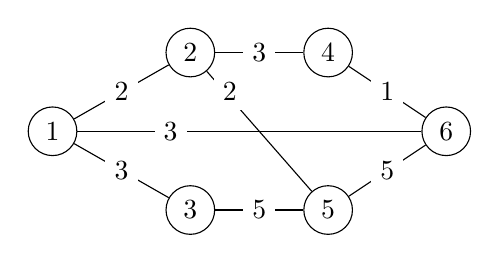
\begin{tikzpicture}
        \draw (0, 0) node[circle, draw](n1) {1};
        \draw (1.75, 1) node[circle, draw](n2) {2};
        \draw (1.75,-1) node[circle, draw](n3) {3};
        \draw (3.5, 1) node[circle, draw](n4) {4};
        \draw (3.5,-1) node[circle, draw](n5) {5};
        \draw (5, 0) node[circle, draw](n6) {6};
        \draw (n1) -- node[fill=white]{2} (n2);
        \draw (n1) -- node[fill=white]{3} (n3);
        \draw (n2) -- node[fill=white]{3} (n4);
        \draw (n4) -- node[fill=white]{1} (n6);
        \draw (n3) -- node[fill=white]{5} (n5);
        \draw (n5) -- node[fill=white]{5} (n6);
        \draw (n1) ++(1.5,0) node[fill=white]{3} (n1) --  (n6);
        \draw (n2) ++(0.5, -0.5) node[fill=white]{2} (n2) -- (n5);
    \end{tikzpicture}
    \caption{Example graph for distance vector calculation}\label{fig:dva_ex}
\end{figure}

\subsubsection{Dijikstra's Algorithm}

\subsubsection{OSI Model}

\subsubsection{TCP/IP}

\subsubsection{TCP - Layer 4 Protocol}

See RFC 793 to read the spec of TCP.

\begin{figure}[H]
    \centering
    \footnotesize
    \begin{varwidth}{\linewidth}
    \begin{verbatim}
     0                   1                   2                   3
     0 1 2 3 4 5 6 7 8 9 0 1 2 3 4 5 6 7 8 9 0 1 2 3 4 5 6 7 8 9 0 1
    +-+-+-+-+-+-+-+-+-+-+-+-+-+-+-+-+-+-+-+-+-+-+-+-+-+-+-+-+-+-+-+-+
    |          Source Port          |       Destination Port        |
    +-+-+-+-+-+-+-+-+-+-+-+-+-+-+-+-+-+-+-+-+-+-+-+-+-+-+-+-+-+-+-+-+
    |                        Sequence Number                        |
    +-+-+-+-+-+-+-+-+-+-+-+-+-+-+-+-+-+-+-+-+-+-+-+-+-+-+-+-+-+-+-+-+
    |                    Acknowledgment Number                      |
    +-+-+-+-+-+-+-+-+-+-+-+-+-+-+-+-+-+-+-+-+-+-+-+-+-+-+-+-+-+-+-+-+
    |  Data |           |U|A|P|R|S|F|                               |
    | Offset| Reserved  |R|C|S|S|Y|I|            Window             |
    |       |           |G|K|H|T|N|N|                               |
    +-+-+-+-+-+-+-+-+-+-+-+-+-+-+-+-+-+-+-+-+-+-+-+-+-+-+-+-+-+-+-+-+
    |           Checksum            |         Urgent Pointer        |
    +-+-+-+-+-+-+-+-+-+-+-+-+-+-+-+-+-+-+-+-+-+-+-+-+-+-+-+-+-+-+-+-+
    |                    Options                    |    Padding    |
    +-+-+-+-+-+-+-+-+-+-+-+-+-+-+-+-+-+-+-+-+-+-+-+-+-+-+-+-+-+-+-+-+
    |                             data                              |
    +-+-+-+-+-+-+-+-+-+-+-+-+-+-+-+-+-+-+-+-+-+-+-+-+-+-+-+-+-+-+-+-+
    \end{verbatim}
    \end{varwidth}
    \caption{TCP Header Format}\label{fig:tcp_header}
\end{figure}

Source Port: 16 bits

    The source port number.

Destination Port: 16 bits

    The desitnation port number.

Sequence Number: 32 bits

    The sequence number of the first data octet in this segment (except
    when SYN is present). If SYN is present the sequence number is the
    initial sequence number (ISN) and the first data octet is ISN+1.

Acknowledgment Number:  32 bits

    If the ACK control bit is set this field contains the value of the
    next sequence number the sender of the segment is expecting to
    receive.  Once a connection is established this is always sent.

Data Offset:  4 bits

    The number of 32 bit words in the TCP Header.  This indicates where
    the data begins.  The TCP header (even one including options) is an
    integral number of 32 bits long.

Reserved:  6 bits

    Reserved for future use.  Must be zero.

Control Bits:  6 bits (from left to right):

    URG:  Urgent Pointer field significant
    ACK:  Acknowledgment field significant
    PSH:  Push Function
    RST:  Reset the connection
    SYN:  Synchronize sequence numbers
    FIN:  No more data from sender

Window:  16 bits

    The number of data octets beginning with the one indicated in the
    acknowledgment field which the sender of this segment is willing to
    accept.

Checksum:  16 bits

    The checksum field is the 16 bit one's complement of the one's
    complement sum of all 16 bit words in the header and text.  If a
    segment contains an odd number of header and text octets to be
    checksummed, the last octet is padded on the right with zeros to
    form a 16 bit word for checksum purposes.  The pad is not
    transmitted as part of the segment.  While computing the checksum,
    the checksum field itself is replaced with zeros.

    The checksum also covers a 96 bit pseudo header conceptually
    prefixed to the TCP header.  This pseudo header contains the Source
    Address, the Destination Address, the Protocol, and TCP length.
    This gives the TCP protection against misrouted segments.  This
    information is carried in the Internet Protocol and is transferred
    across the TCP/Network interface in the arguments or results of
    calls by the TCP on the IP.

\subsubsection{UDP - Layer 4 Protocol}

\begin{figure}[H]
    \centering
    \footnotesize
    \begin{varwidth}{\linewidth}
    \begin{verbatim}
     0                   1                   2                   3
     0 1 2 3 4 5 6 7 8 9 0 1 2 3 4 5 6 7 8 9 0 1 2 3 4 5 6 7 8 9 0 1
    +-+-+-+-+-+-+-+-+-+-+-+-+-+-+-+-+-+-+-+-+-+-+-+-+-+-+-+-+-+-+-+-+
    |                      Source IPv4 Address                      |
    +-+-+-+-+-+-+-+-+-+-+-+-+-+-+-+-+-+-+-+-+-+-+-+-+-+-+-+-+-+-+-+-+
    |                   Destination IPv4 Address                    |
    +-+-+-+-+-+-+-+-+-+-+-+-+-+-+-+-+-+-+-+-+-+-+-+-+-+-+-+-+-+-+-+-+
    |     Zeros     |    Protocol   |         UDP Length            |
    +-+-+-+-+-+-+-+-+-+-+-+-+-+-+-+-+-+-+-+-+-+-+-+-+-+-+-+-+-+-+-+-+
    |          Source Port          |      Destination Port         |
    +-+-+-+-+-+-+-+-+-+-+-+-+-+-+-+-+-+-+-+-+-+-+-+-+-+-+-+-+-+-+-+-+
    |                             Data                              |
    +-+-+-+-+-+-+-+-+-+-+-+-+-+-+-+-+-+-+-+-+-+-+-+-+-+-+-+-+-+-+-+-+
    \end{verbatim}
    \end{varwidth}
    \caption{UDP Header Format}\label{fig:udp_header}
\end{figure}

\subsubsection{ARP - Layer 3 Protocol}

\subsubsection{IP - Layer 3 Protocol}

\begin{figure}[H]
    \centering
    \footnotesize
    \begin{varwidth}{\linewidth}
    \begin{verbatim}
     0                   1                   2                   3
     0 1 2 3 4 5 6 7 8 9 0 1 2 3 4 5 6 7 8 9 0 1 2 3 4 5 6 7 8 9 0 1
    +-+-+-+-+-+-+-+-+-+-+-+-+-+-+-+-+-+-+-+-+-+-+-+-+-+-+-+-+-+-+-+-+
    |Version|  IHL  |Type of Service|          Total Length         |
    +-+-+-+-+-+-+-+-+-+-+-+-+-+-+-+-+-+-+-+-+-+-+-+-+-+-+-+-+-+-+-+-+
    |         Identification        |Flags|      Fragment Offset    |
    +-+-+-+-+-+-+-+-+-+-+-+-+-+-+-+-+-+-+-+-+-+-+-+-+-+-+-+-+-+-+-+-+
    |  Time to Live |    Protocol   |         Header Checksum       |
    +-+-+-+-+-+-+-+-+-+-+-+-+-+-+-+-+-+-+-+-+-+-+-+-+-+-+-+-+-+-+-+-+
    |                       Source Address                          |
    +-+-+-+-+-+-+-+-+-+-+-+-+-+-+-+-+-+-+-+-+-+-+-+-+-+-+-+-+-+-+-+-+
    |                    Destination Address                        |
    +-+-+-+-+-+-+-+-+-+-+-+-+-+-+-+-+-+-+-+-+-+-+-+-+-+-+-+-+-+-+-+-+
    |                    Options                    |    Padding    |
    +-+-+-+-+-+-+-+-+-+-+-+-+-+-+-+-+-+-+-+-+-+-+-+-+-+-+-+-+-+-+-+-+
    \end{verbatim}
    \end{varwidth}
    \caption{IPv4 header format}\label{fig:ipv4_header}
\end{figure}

\subsubsection{ICMP - Layer 3 Protocol}

Support protocol used by network devices to send error messages and operational
information indicating success or failure when comunicating with another IP
address.\cite{wiki:icmp} Example of operational information are

\begin{itemize}
    \item Ping: This utility is implemented using the ICMP echo request and echo
          reply messages.
    \item Destination Unreachable: Used to report that an IP datagram could not
          be delivered.
    \item Redirect: Report an incorrect route or use another path.
    \item Time Exceeded: Fragment failed to arrive or TTL field in IP header
          reached zero.
\end{itemize}

Figure \ref{fig:icmp} shows ICMP packet that contains, type, code checksum and
rest of header.

\begin{figure}[H]
    \centering
    \footnotesize
    \begin{varwidth}{\linewidth}
    \begin{verbatim}
     0                   1                   2                   3
     0 1 2 3 4 5 6 7 8 9 0 1 2 3 4 5 6 7 8 9 0 1 2 3 4 5 6 7 8 9 0 1
    +-+-+-+-+-+-+-+-+-+-+-+-+-+-+-+-+-+-+-+-+-+-+-+-+-+-+-+-+-+-+-+-+
    |     Type      |     Code      |          Checksum             |
    +-+-+-+-+-+-+-+-+-+-+-+-+-+-+-+-+-+-+-+-+-+-+-+-+-+-+-+-+-+-+-+-+
    |                             unused                            |
    +-+-+-+-+-+-+-+-+-+-+-+-+-+-+-+-+-+-+-+-+-+-+-+-+-+-+-+-+-+-+-+-+
    |      Internet Header + 64 bits of Original Data Datagram      |
    +-+-+-+-+-+-+-+-+-+-+-+-+-+-+-+-+-+-+-+-+-+-+-+-+-+-+-+-+-+-+-+-+
    \end{verbatim}
    \end{varwidth}
    \caption{ICMP header format}\label{fig:icmp}
\end{figure}

\begin{itemize}
    \item Type: ICMP type, this is the ICMP Control Messages.
    \item Code: Each ICMP type contains subtype.
    \item Checksum: checksum of the ICMP header and data with value 0 subtituded for this field.
    \item Rest of header: Four-byte field, contents vary based on the ICMP type and code.
\end{itemize}

\subsubsection{Ethernet - Layer 2 Protocol}

Ethernet frame is a data link protocol data unit and uses the underlying
physical layer transport mechanism.\cite{wiki:ethernet_frame}

\begin{figure}[H]
    \centering
    \footnotesize
    \begin{varwidth}{\linewidth}
    \begin{verbatim}
    +-+-+-+-+-+-+-+-+-+-+-+-+-+-+-+-+-+-+-+-+--+-+-+-+-+-+-+-+-+-+-+-+-+-+-+-+-+-+-+
    |     Preamble (7 bytes)     |     SFP (1 byte)    | MAC destination (6 bytes) |
    +-+-+-+-+-+-+-+-+-+-+-+-+-+-+-+-+-+-+-+-+--+-+-+-+-+-+-+-+-+-+-+-+-+-+-+-+-+-+-+
    |   MAC source (6 bytes)     | Ehtertype (2 bytes) | Payload (42-1500 bytes)   |
    +-+-+-+-+-+-+-+-+-+-+-+-+-+-+-+-+-+-+-+-+--+-+-+-+-+-+-+-+-+-+-+-+-+-+-+-+-+-+-+
    |             CRC (4 bytes)  |            IPG  (12 bytes)                      |
    +-+-+-+-+-+-+-+-+-+-+-+-+-+-+-+-+-+-+-+-+--+-+-+-+-+-+-+-+-+-+-+-+-+-+-+-+-+-+-+
    \end{verbatim}
    \end{varwidth}
    \caption{Ethernet Frame}\label{fig:ethernet_frame}
\end{figure}

\subsubsection{Network Classification}

\subsubsection{Subnet}

\subsubsection{Network Address Translation (NAT)}

\subsubsection{CSMA/CD}

Carrier Sense Multiple Access with Collision Detection is a protocol used in
Ethernet networks to regulate the transmission of data packets to avoid
collisions.\cite{wiki:csmacd}

\begin{enumerate}
    \item Carrier Sense (CS): Before sending data, a device checks the network
          to see if any other device is currently transmitting. If the network
          is clear, the device proceeds to transmit its data. If it detects that
          another device is already transmitting, it waits for the transmission
          to finish.
    \item Multiple Access (MA): Multiple devices share the same network medium
          (like a cable), and they all have equal access to it. This means that
          multiple devices can attempt to transmit data on the network
          simultaneously.
    \item Collision Detection (CD): If two devices happen to transmit data at
          the same time, causing a collision, they detect the collision and take
          steps to resolve it. When a collision is detected, the transmitting
          devices stop sending data and wait for a random amount of time before
          attempting to transmit again. This random backoff period helps to
          reduce the likelihood of another collision occurring immediately after
          the first one.
\end{enumerate}

\newpage
\printbibliography
\end{document}

